%----------------------------------------------------------------------------------------
%	Section: Viewer Features
%----------------------------------------------------------------------------------------
\section{Viewer Features}

\begin{figure}[h]
    	\centering
    		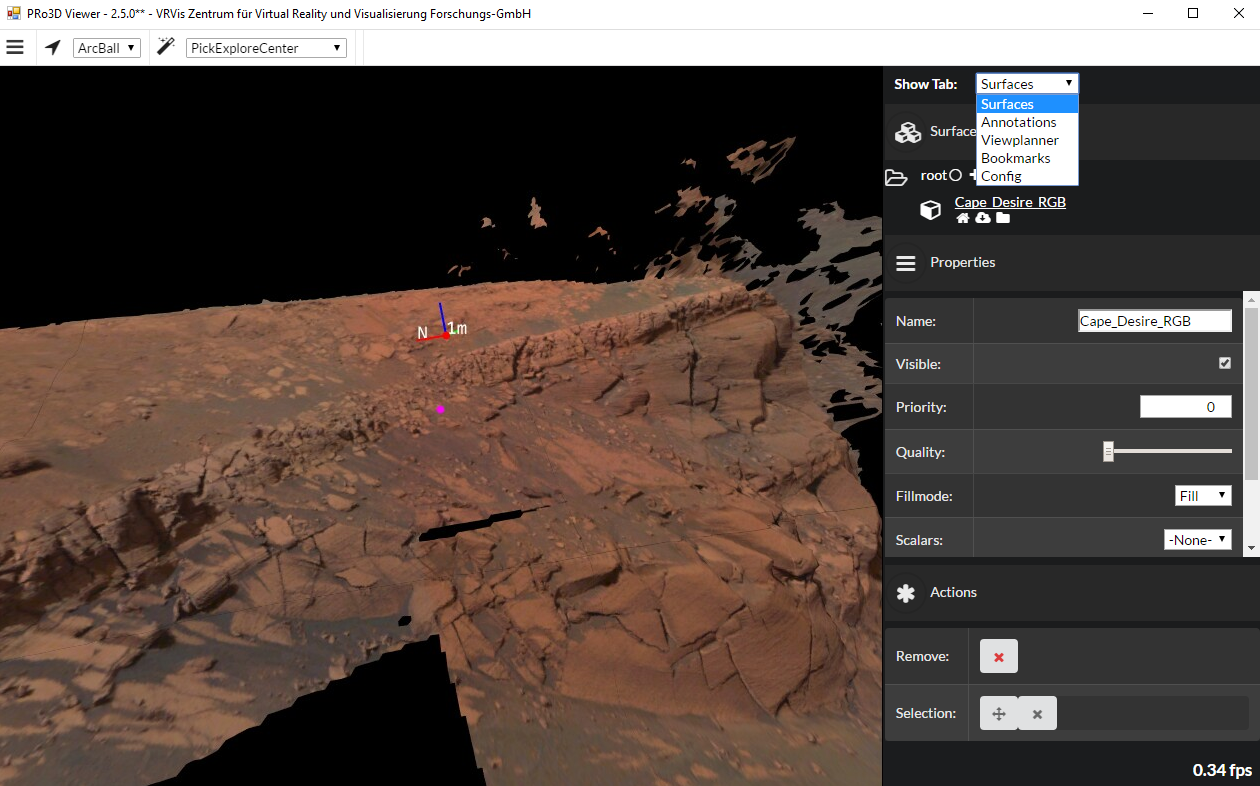
\includegraphics[width=1\textwidth]{pics/featureMenu.png}
    	\caption[Viewer Features]{There are menu tabs (right) for each feature in the viewer.}
    	\label{fig:featureMenu}
   \end{figure}
	
The feature tabs show a list of the respective features, the properties of the selected feature from this list and some actions for this feature.
For surfaces, annotations and bookmarks it is possible to group them, as described in Section~\ref{sec:grouping}.
%----------------------------------------------------------------------------------------
%	SubSection: Surfaces
%----------------------------------------------------------------------------------------
\subsection{Surfaces}
\label{sec:surfaces}

\begin{figure}[h]
    	\centering
    		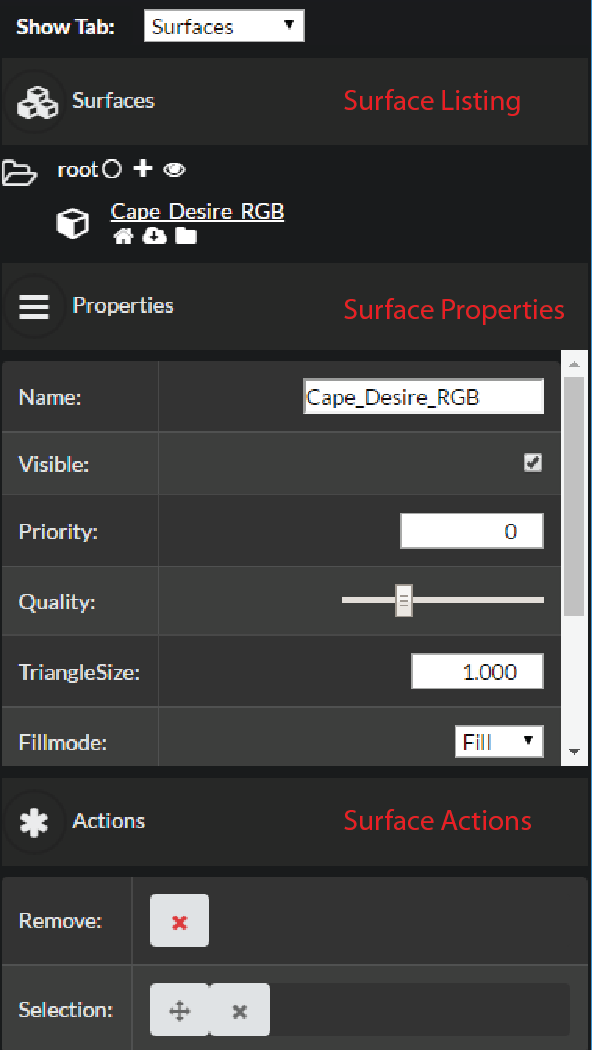
\includegraphics[width=0.5\textwidth]{pics/SurfacesAI.png}
    	\caption[Viewer Features Surfaces]{The surfaces tab.}
    	\label{fig:surfaces}
   \end{figure}

The listing shows all surfaces in the scene. You can classify them in any group and subgroup layers, described in Section~\ref{sec:grouping}.
You can select a surface by clicking on the surface's name. Then you can see the surface's properties in the properties panel and use the actions in the actions panel. 
It is also possible to select multiple surfaces by clicking the square icon in front of each surface. The selected surfaces have a green square in the list. The multiselection is used to move one ore more surfaces from one group to the active group.
Under the surface's name is a little menu:
\begin{itemize}
	\item \textit{FlyTo}: A click on the button triggers a FlyTo animation.
	\item \textit{portable}: This creates a folder hierarchy as used in the old viewer version. A scene file is created and the surfaces are copied to the surface folder.
	\item \textit{openFolder}: Opens the folder where the scene file resides.	
\end{itemize}

In the surface properties panel are some adjustments possible:
\begin{itemize}
	\item \textit{Name}: The surface's name. You can change it in the text field and press ``enter''.
	\item \textit{Visible}: The surface is visible (checked) or not (unchecked).
	\item \textit{Priority}:  Often multiple surfaces are available for a certain area on the planet surface. These surfaces represent the same piece of ground and typically overlap. This parameter allows to assign a priority to a surface to tell the graphics card which surface should be rendered in front. Lower numbers mean a higher priority in rendering, with 0 being the highest priority. You can also give the highest priority surface a ranking of, for instance, 0.1 (= 10cm) to make annotations more visible. The priority can be dynamically changed via the surface properties so you can try out what works best.
	\item \textit{Quality}: 
	\item \textit{TriangleSize}:
	\item \textit{FillMode}: You can switch between solid/ wireframe/ point rendering of the geometry.
	\item \textit{Scalars}:
	\item \textit{Textures}:
	\item \textit{Cull Faces}:
\end{itemize}

The surfaces actions are described in Section~\ref{sec:leafActions}.
%----------------------------------------------------------------------------------------
%	SubSection: Annotations
%----------------------------------------------------------------------------------------
\subsection{Annotations}
\label{sec:annotations}

\begin{figure}[h]
    	\centering
    		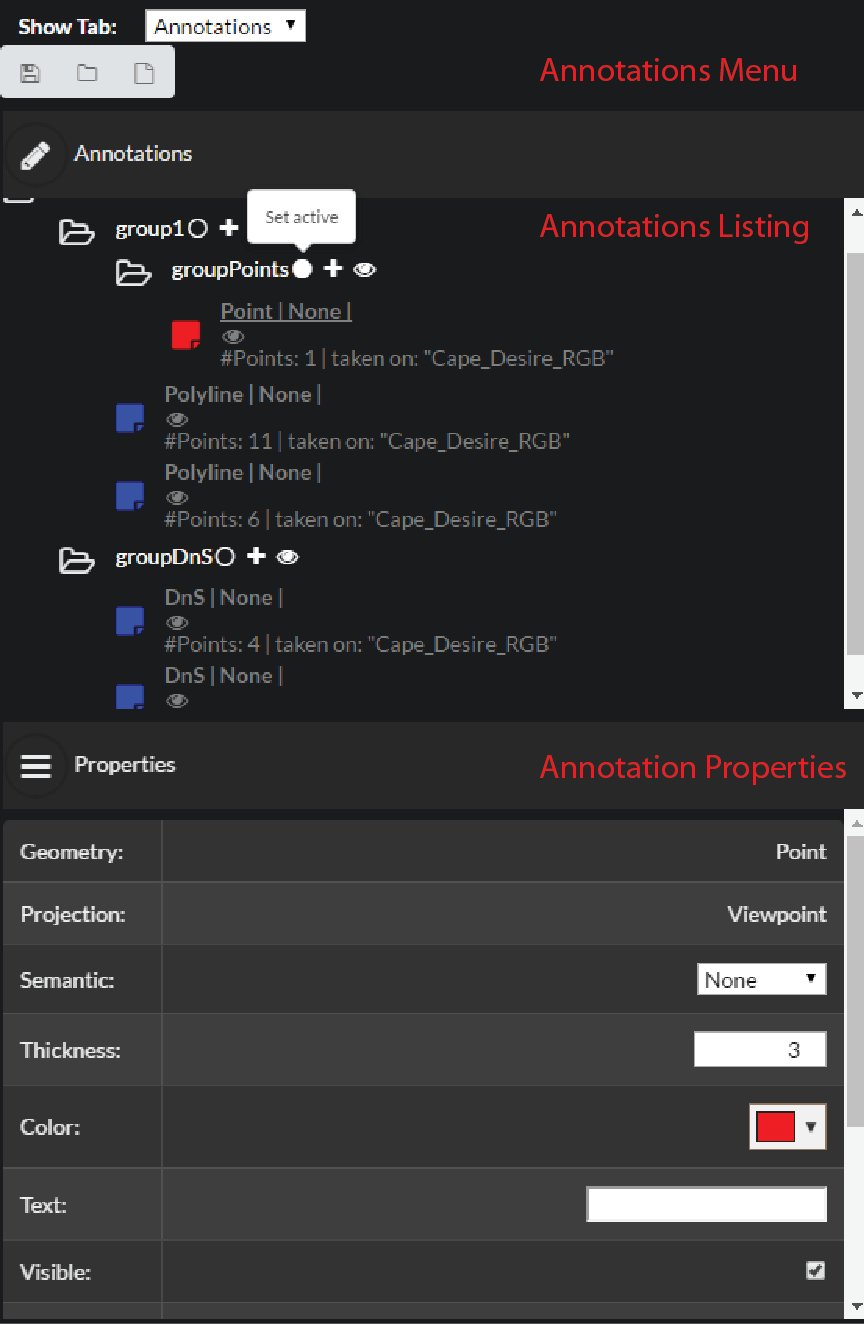
\includegraphics[width=0.5\textwidth]{pics/AnnotationsTabAI.png}
    	\caption[Viewer Features Annotations]{The annotations tab.}
    	\label{fig:annoProps}
   \end{figure}
	
The annotations tab consists of four parts (Figure~\ref{fig:annoProps}):

%----------------------------------------------------------------------------------------Annotations menu
\subsubsection{Annotations Menu}

In contrast to all other viewer features, the annotations are NOT saved in the scene file!
There is a separate menu on top of the annotations tab:
\begin{itemize}
	\item \textit{Save Annotations}: Opens a ``Save As'' window. Give your annotations xml file a name and click the ``Save'' button.
	\item \textit{Load Annotations}: Select the annotations xml file and press the ``Open'' button. 
	\item \textit{Clear Annotation List}: This clears the whole annotation list.
\end{itemize}

%----------------------------------------------------------------------------------------Annotations listing
\subsubsection{Annotations Listing}

The listing shows all annotations in the scene. You can classify them in any group and subgroup layers, described in Section~\ref{sec:grouping}.
You can select an annotation by clicking on the annotation's name. Then you can see the annotation's properties in the properties panel and use the actions in the actions panel. 
It is also possible to select more annotations by clicking the square icon in front of each annotation. The selected annotations have a green color in the viewer and a green square in the list. The multiselection is used to move one ore more annotations from one group to the active group.

%----------------------------------------------------------------------------------------Annotations properties
\subsubsection{Annotations Properties}

The properties of the selected annotation (click on annotation's name) are shown. There you can get information and change some of the settings:
\begin{itemize}
	\item \textit{Geometry}: Shows the annotation mode (described in Section~\ref{sec:drawAnnotation}). This is not changeable retrospectively.
	\item \textit{Projection}: Shows the projection which determines the direction of the picking ray (described in Section~\ref{sec:drawAnnotation}, shown in Figure~\ref{fig:projection}). This is not changeable retrospectively.
	\item \textit{Semantic}: 
	\item \textit{Thickness}: You can change the annotation's line thickness.
	\item \textit{Color}: You can change the annotation's color.
	\item \textit{Text}: You can append a note. Write in the text field and press ``Enter''. The note will appear next to the annotation in the viewer. 
	\item \textit{Visible}: The annotation is visible (checked) or not (unchecked).
	\item \textit{ShowDnS}: For each annotation with more than three picking points Dip and Strike information (Section~\ref{sec:drawAnnotation}) is available. The DnS is visible (checked) or not (unchecked).
	\item \textit{Height}:  The height between the annotation's start and end point.
	\item \textit{HeightDelta}: The height difference between the highest and lowest point of the projected line.
	\item \textit{Length}: The sum of direct distances between the picking points.
	\item \textit{WayLength}: The sum of projected distances between the picking points.
\end{itemize}

The annotations actions are described in Section~\ref{sec:leafActions}.

%----------------------------------------------------------------------------------------Import AnnotationGroups
\subsubsection{Import Annotations from old viewer versions} 

To import annotations from old scene files click the ``browse'' button in the \textbf{ImportAnnotationGroups} section in the Scene Menu (Figure~\ref{fig:StartMenu}). This opens a folder browser dialog, where you can select an old scene file an click ''Open''.
The annotations are loaded in the same group hierarchy to the ``root'' group.


%----------------------------------------------------------------------------------------
%	SubSection: ViewPlanner
%----------------------------------------------------------------------------------------
%\subsection{ViewPlanner}
%\label{sec:viewPlanner}

%----------------------------------------------------------------------------------------
%	SubSection: Bookmarks
%----------------------------------------------------------------------------------------
\subsection{Bookmarks}
\label{sec:bookmarks}

\begin{figure}[h]
    	\centering
    		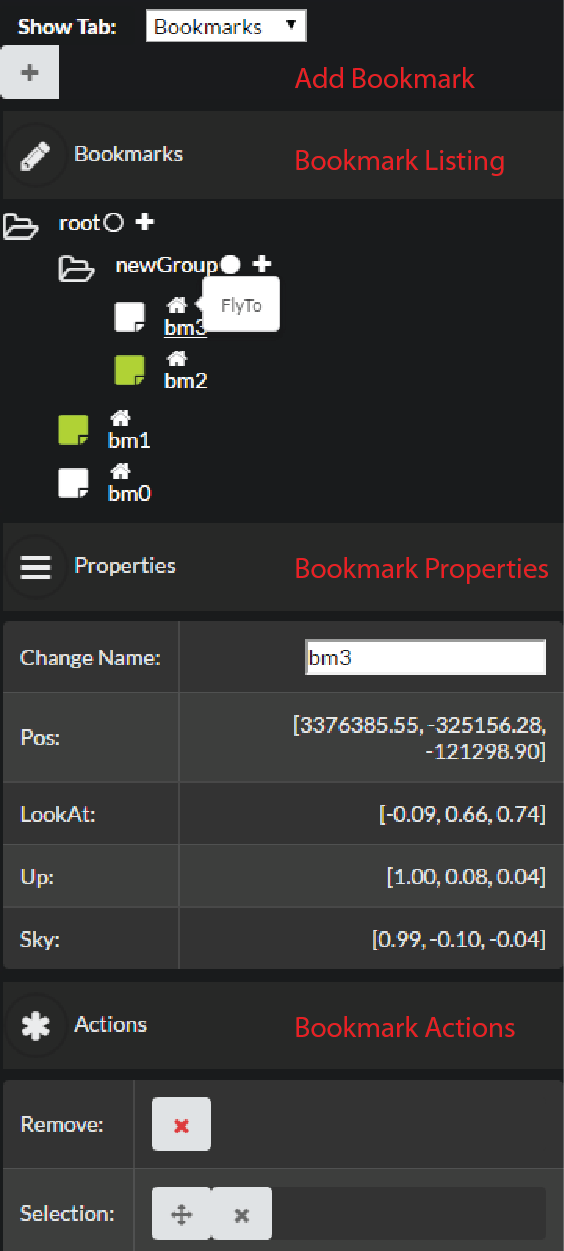
\includegraphics[width=0.5\textwidth]{pics/bookmarks.png}
    	\caption[Viewer Features Bookmarks]{The bookmarks tab.}
    	\label{fig:bookmarks}
   \end{figure}
	
Bookmarks enable the user to record a certain camera viewpoint.
To add a new bookmark click the ``+'' button on top of the tab (Figure~\ref{fig:bookmarks}). The new bookmark is added to the active group in the bookmarks listing.
To view the bookmark's properties and actions click on the bookmark's name. Clicking the ``house'' button beside the bookmark's name triggers a FlyTo. For multiselection click on the bookmark's square icons.

%----------------------------------------------------------------------------------------
%	SubSection: Viewer Configuration
%----------------------------------------------------------------------------------------
\subsection{Viewer Configuration}
\label{sec:config}

\begin{figure}[h]
    	\centering
    		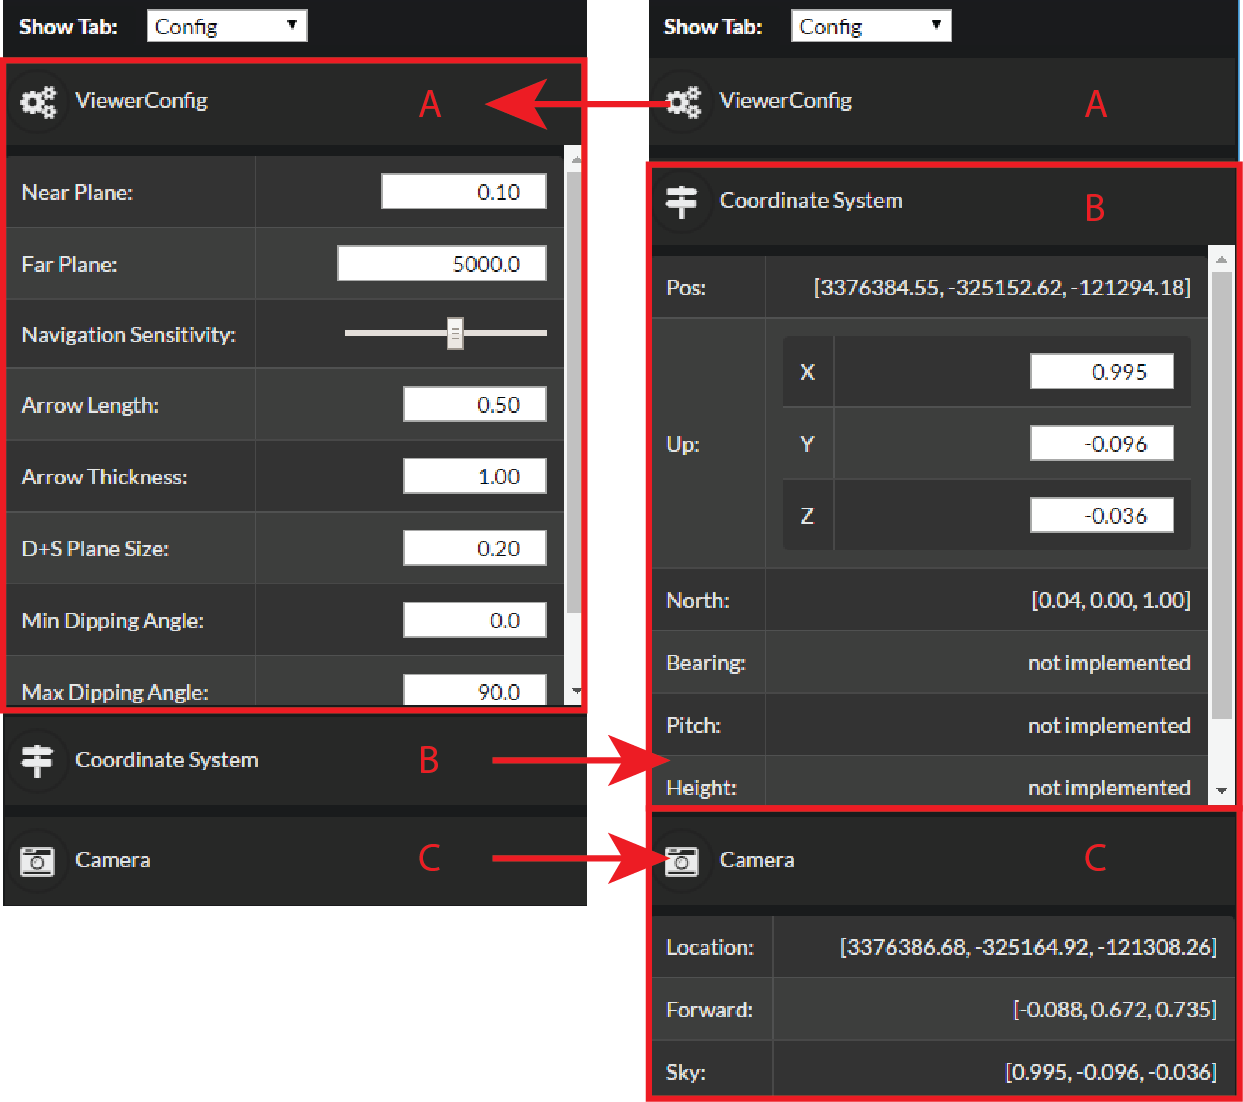
\includegraphics[width=0.8\textwidth]{pics/ViewerConfigAI.png}
    	\caption[Viewer Configuration]{The ``Config'' Menu with the ViewerConfiguration (A), Coordinate System (B) and Camera settings (C).}
    	\label{fig:viewerConfig}
   \end{figure}

To edit the viewer properties, select ``Config'' in the viewer features drop down menu (Figure~\ref{fig:featureMenu}).
There are three submenus in the config tab:
\begin{itemize}
	\item ViewerConfig (A in Figure~\ref{fig:viewerConfig})
	\item Coordinate System (B in Figure~\ref{fig:viewerConfig})
	\item Camera (C in Figure~\ref{fig:viewerConfig})
\end{itemize}

%----------------------------------------------------------------------------------------Viewer Config
\subsubsection{ViewerConfig} 

A set of major viewer properties can be adjusted:
\begin{itemize}
	\item \textit{Near/Far Plane}: The near- and the far clipping plane are automatically adjusted according to the data to be rendered. The set values are shown in the config panel and can be adjusted afterwards. 
	\item \textit{Navigation Sensitivity}: The navigation sensitivity can also be adjusted by PageUp and PageDown keys. 
	\item \textit{Arrow Length/Thickness}: The arrow length and thickness is set for up- and north vectors, dip and strike vectors and the up- and lookAt vectors in the rover view planner. 
	\item \textit{D+S Plane Size}: The dip and strike measurements plane size, described in Section~\ref{sec:drawAnnotation}
 (Figure~\ref{fig:drawAnnotations}).
	\item \textit{Min/Max Dipping Angle}: The dip and strike measurements dipping angle range. The dipping angle is coded into the color of the disc and arrow of a measurement (Figure~\ref{fig:drawAnnotations}).
	\item \textit{Lod Colors}: The different levels of detail of the surface geometry can be colored in different shades of red.
			This helps to evaluate the export of OPC data.
\end{itemize}

%----------------------------------------------------------------------------------------Coordinate System
\subsubsection{Coordinate System} 

The coordinate system menu shows the position, Up- and North Vector of the coordinate system described in Section~\ref{sec:placeCS}, shown in Figure~\ref{fig:coordinateSystem}.
The Up- and the North Vector are used for the projection measurements (Figure~\ref{fig:drawAnnotations}). Initially the Up Vector's direction is set in the positive z-direction and the North Vector's in the positive y-direction. But you can manipulate the Up Vector manually for different data. Both vectors are computed automatically with picking of a new position for the coordinate system. The north vector is further relevant for bearing measurements. % and the rover placement in the View Planner (see Section 4.6). 

%----------------------------------------------------------------------------------------Camera
\subsubsection{Camera} 

The Camera submenu shows the Location, Forward- and Sky vector of the main camera.
%----------------------------------------------------------------------------------------
%	SubSection: Grouping
%----------------------------------------------------------------------------------------
\subsection{Grouping}
\label{sec:grouping}

\begin{figure}[h]
    	\centering
    		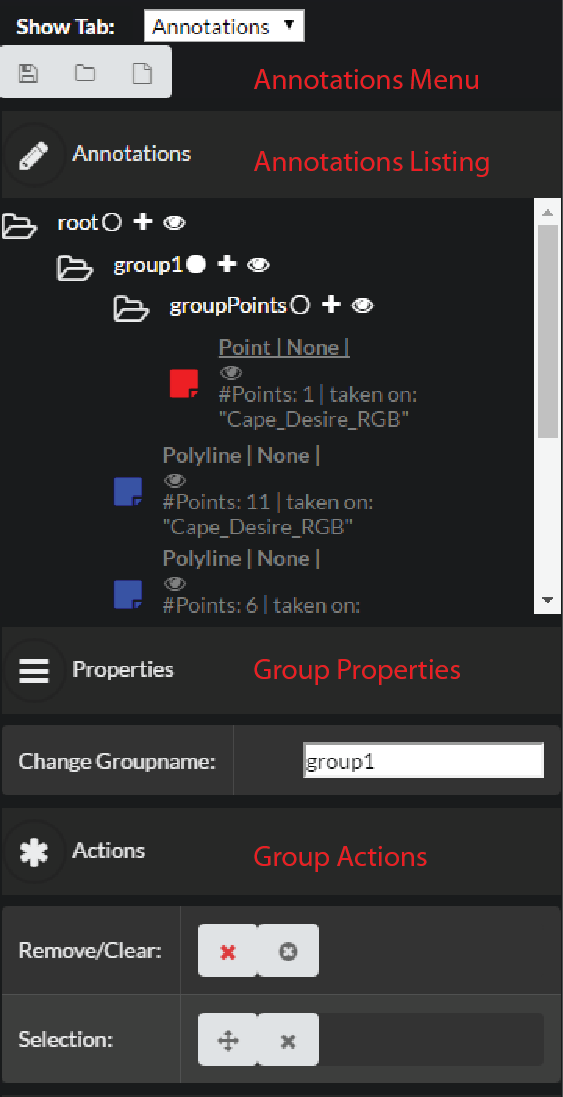
\includegraphics[width=0.5\textwidth]{pics/GroupsProperties.png}
    	\caption[Viewer Features]{The group properties and actions.}
    	\label{fig:groupProps}
   \end{figure}

Grouping is possible for surfaces, annotations and bookmarks.
The ``root'' group is the highest level where you can add leafs and subgroups (Figure~\ref{fig:groupProps}).
Each group has a context menu:
\begin{itemize}
	\item \textit{Set Active}: The active group gets the new leaf. Per default the ``root'' is active.
	\item \textit{Add Group}: Adds a new and empty subgroup.
	\item \textit{Toggle Group}: Sets all leafs in this group and its subgroups invisible.
\end{itemize}

%----------------------------------------------------------------------------------------Group actions
\subsubsection{Group Actions}
\label{sec:groupActions}

\begin{itemize}
	\item \textit{Remove}: Removes the group with all its leafs and subgroups.
	\item \textit{Clear}: Removes all leafs and subgroups from group but retains the empty group. 
	\item \textit{Selection: Move}: Moves all selected leafs (green squares) to the active group.
	\item \textit{Selection: Clear}: Clears the selection (the leafs were not removed).
\end{itemize}
	
%----------------------------------------------------------------------------------------Leaf actions
\subsubsection{Leaf Actions}
\label{sec:leafActions}

\begin{itemize}
	\item \textit{Remove}: Removes the leaf.
	\item \textit{Selection: Move}: Moves all selected leafs (green squares) to the active group.
	\item \textit{Selection: Clear}: Clears the selection (the leafs were not removed).
\end{itemize}
